% Options for packages loaded elsewhere
\PassOptionsToPackage{unicode}{hyperref}
\PassOptionsToPackage{hyphens}{url}
%
\documentclass[
  9pt,
]{article}
\usepackage{amsmath,amssymb}
\usepackage{lmodern}
\usepackage{iftex}
\ifPDFTeX
  \usepackage[T1]{fontenc}
  \usepackage[utf8]{inputenc}
  \usepackage{textcomp} % provide euro and other symbols
\else % if luatex or xetex
  \usepackage{unicode-math}
  \defaultfontfeatures{Scale=MatchLowercase}
  \defaultfontfeatures[\rmfamily]{Ligatures=TeX,Scale=1}
\fi
% Use upquote if available, for straight quotes in verbatim environments
\IfFileExists{upquote.sty}{\usepackage{upquote}}{}
\IfFileExists{microtype.sty}{% use microtype if available
  \usepackage[]{microtype}
  \UseMicrotypeSet[protrusion]{basicmath} % disable protrusion for tt fonts
}{}
\makeatletter
\@ifundefined{KOMAClassName}{% if non-KOMA class
  \IfFileExists{parskip.sty}{%
    \usepackage{parskip}
  }{% else
    \setlength{\parindent}{0pt}
    \setlength{\parskip}{6pt plus 2pt minus 1pt}}
}{% if KOMA class
  \KOMAoptions{parskip=half}}
\makeatother
\usepackage{xcolor}
\usepackage[margin=1in]{geometry}
\usepackage{color}
\usepackage{fancyvrb}
\newcommand{\VerbBar}{|}
\newcommand{\VERB}{\Verb[commandchars=\\\{\}]}
\DefineVerbatimEnvironment{Highlighting}{Verbatim}{commandchars=\\\{\}}
% Add ',fontsize=\small' for more characters per line
\usepackage{framed}
\definecolor{shadecolor}{RGB}{248,248,248}
\newenvironment{Shaded}{\begin{snugshade}}{\end{snugshade}}
\newcommand{\AlertTok}[1]{\textcolor[rgb]{0.94,0.16,0.16}{#1}}
\newcommand{\AnnotationTok}[1]{\textcolor[rgb]{0.56,0.35,0.01}{\textbf{\textit{#1}}}}
\newcommand{\AttributeTok}[1]{\textcolor[rgb]{0.77,0.63,0.00}{#1}}
\newcommand{\BaseNTok}[1]{\textcolor[rgb]{0.00,0.00,0.81}{#1}}
\newcommand{\BuiltInTok}[1]{#1}
\newcommand{\CharTok}[1]{\textcolor[rgb]{0.31,0.60,0.02}{#1}}
\newcommand{\CommentTok}[1]{\textcolor[rgb]{0.56,0.35,0.01}{\textit{#1}}}
\newcommand{\CommentVarTok}[1]{\textcolor[rgb]{0.56,0.35,0.01}{\textbf{\textit{#1}}}}
\newcommand{\ConstantTok}[1]{\textcolor[rgb]{0.00,0.00,0.00}{#1}}
\newcommand{\ControlFlowTok}[1]{\textcolor[rgb]{0.13,0.29,0.53}{\textbf{#1}}}
\newcommand{\DataTypeTok}[1]{\textcolor[rgb]{0.13,0.29,0.53}{#1}}
\newcommand{\DecValTok}[1]{\textcolor[rgb]{0.00,0.00,0.81}{#1}}
\newcommand{\DocumentationTok}[1]{\textcolor[rgb]{0.56,0.35,0.01}{\textbf{\textit{#1}}}}
\newcommand{\ErrorTok}[1]{\textcolor[rgb]{0.64,0.00,0.00}{\textbf{#1}}}
\newcommand{\ExtensionTok}[1]{#1}
\newcommand{\FloatTok}[1]{\textcolor[rgb]{0.00,0.00,0.81}{#1}}
\newcommand{\FunctionTok}[1]{\textcolor[rgb]{0.00,0.00,0.00}{#1}}
\newcommand{\ImportTok}[1]{#1}
\newcommand{\InformationTok}[1]{\textcolor[rgb]{0.56,0.35,0.01}{\textbf{\textit{#1}}}}
\newcommand{\KeywordTok}[1]{\textcolor[rgb]{0.13,0.29,0.53}{\textbf{#1}}}
\newcommand{\NormalTok}[1]{#1}
\newcommand{\OperatorTok}[1]{\textcolor[rgb]{0.81,0.36,0.00}{\textbf{#1}}}
\newcommand{\OtherTok}[1]{\textcolor[rgb]{0.56,0.35,0.01}{#1}}
\newcommand{\PreprocessorTok}[1]{\textcolor[rgb]{0.56,0.35,0.01}{\textit{#1}}}
\newcommand{\RegionMarkerTok}[1]{#1}
\newcommand{\SpecialCharTok}[1]{\textcolor[rgb]{0.00,0.00,0.00}{#1}}
\newcommand{\SpecialStringTok}[1]{\textcolor[rgb]{0.31,0.60,0.02}{#1}}
\newcommand{\StringTok}[1]{\textcolor[rgb]{0.31,0.60,0.02}{#1}}
\newcommand{\VariableTok}[1]{\textcolor[rgb]{0.00,0.00,0.00}{#1}}
\newcommand{\VerbatimStringTok}[1]{\textcolor[rgb]{0.31,0.60,0.02}{#1}}
\newcommand{\WarningTok}[1]{\textcolor[rgb]{0.56,0.35,0.01}{\textbf{\textit{#1}}}}
\usepackage{graphicx}
\makeatletter
\def\maxwidth{\ifdim\Gin@nat@width>\linewidth\linewidth\else\Gin@nat@width\fi}
\def\maxheight{\ifdim\Gin@nat@height>\textheight\textheight\else\Gin@nat@height\fi}
\makeatother
% Scale images if necessary, so that they will not overflow the page
% margins by default, and it is still possible to overwrite the defaults
% using explicit options in \includegraphics[width, height, ...]{}
\setkeys{Gin}{width=\maxwidth,height=\maxheight,keepaspectratio}
% Set default figure placement to htbp
\makeatletter
\def\fps@figure{htbp}
\makeatother
\setlength{\emergencystretch}{3em} % prevent overfull lines
\providecommand{\tightlist}{%
  \setlength{\itemsep}{0pt}\setlength{\parskip}{0pt}}
\setcounter{secnumdepth}{-\maxdimen} % remove section numbering
\ifLuaTeX
\usepackage[bidi=basic]{babel}
\else
\usepackage[bidi=default]{babel}
\fi
\babelprovide[main,import]{ngerman}
% get rid of language-specific shorthands (see #6817):
\let\LanguageShortHands\languageshorthands
\def\languageshorthands#1{}
\ifLuaTeX
  \usepackage{selnolig}  % disable illegal ligatures
\fi
\IfFileExists{bookmark.sty}{\usepackage{bookmark}}{\usepackage{hyperref}}
\IfFileExists{xurl.sty}{\usepackage{xurl}}{} % add URL line breaks if available
\urlstyle{same} % disable monospaced font for URLs
\hypersetup{
  pdftitle={Pendel},
  pdfauthor={Milena Mensching, Justus Weyers},
  pdflang={de},
  hidelinks,
  pdfcreator={LaTeX via pandoc}}

\title{Pendel}
\author{Milena Mensching, Justus Weyers}
\date{2022-12-08}

\begin{document}
\maketitle

\hypertarget{versuch-1}{%
\section{Versuch 1}\label{versuch-1}}

\hypertarget{thema}{%
\subsection{Thema}\label{thema}}

Bestimmung der Wärmekapazität eines Kaloriemeters. Dieses soll in
Versuch 2 dafür verwendet werden, die spezifische Wärmekapazität zweier
Metalle zu bestimmen.

\hypertarget{versuchsaufbau-und-durchfuxfchrung}{%
\subsection{Versuchsaufbau und
Durchführung}\label{versuchsaufbau-und-durchfuxfchrung}}

\begin{figure}
\centering
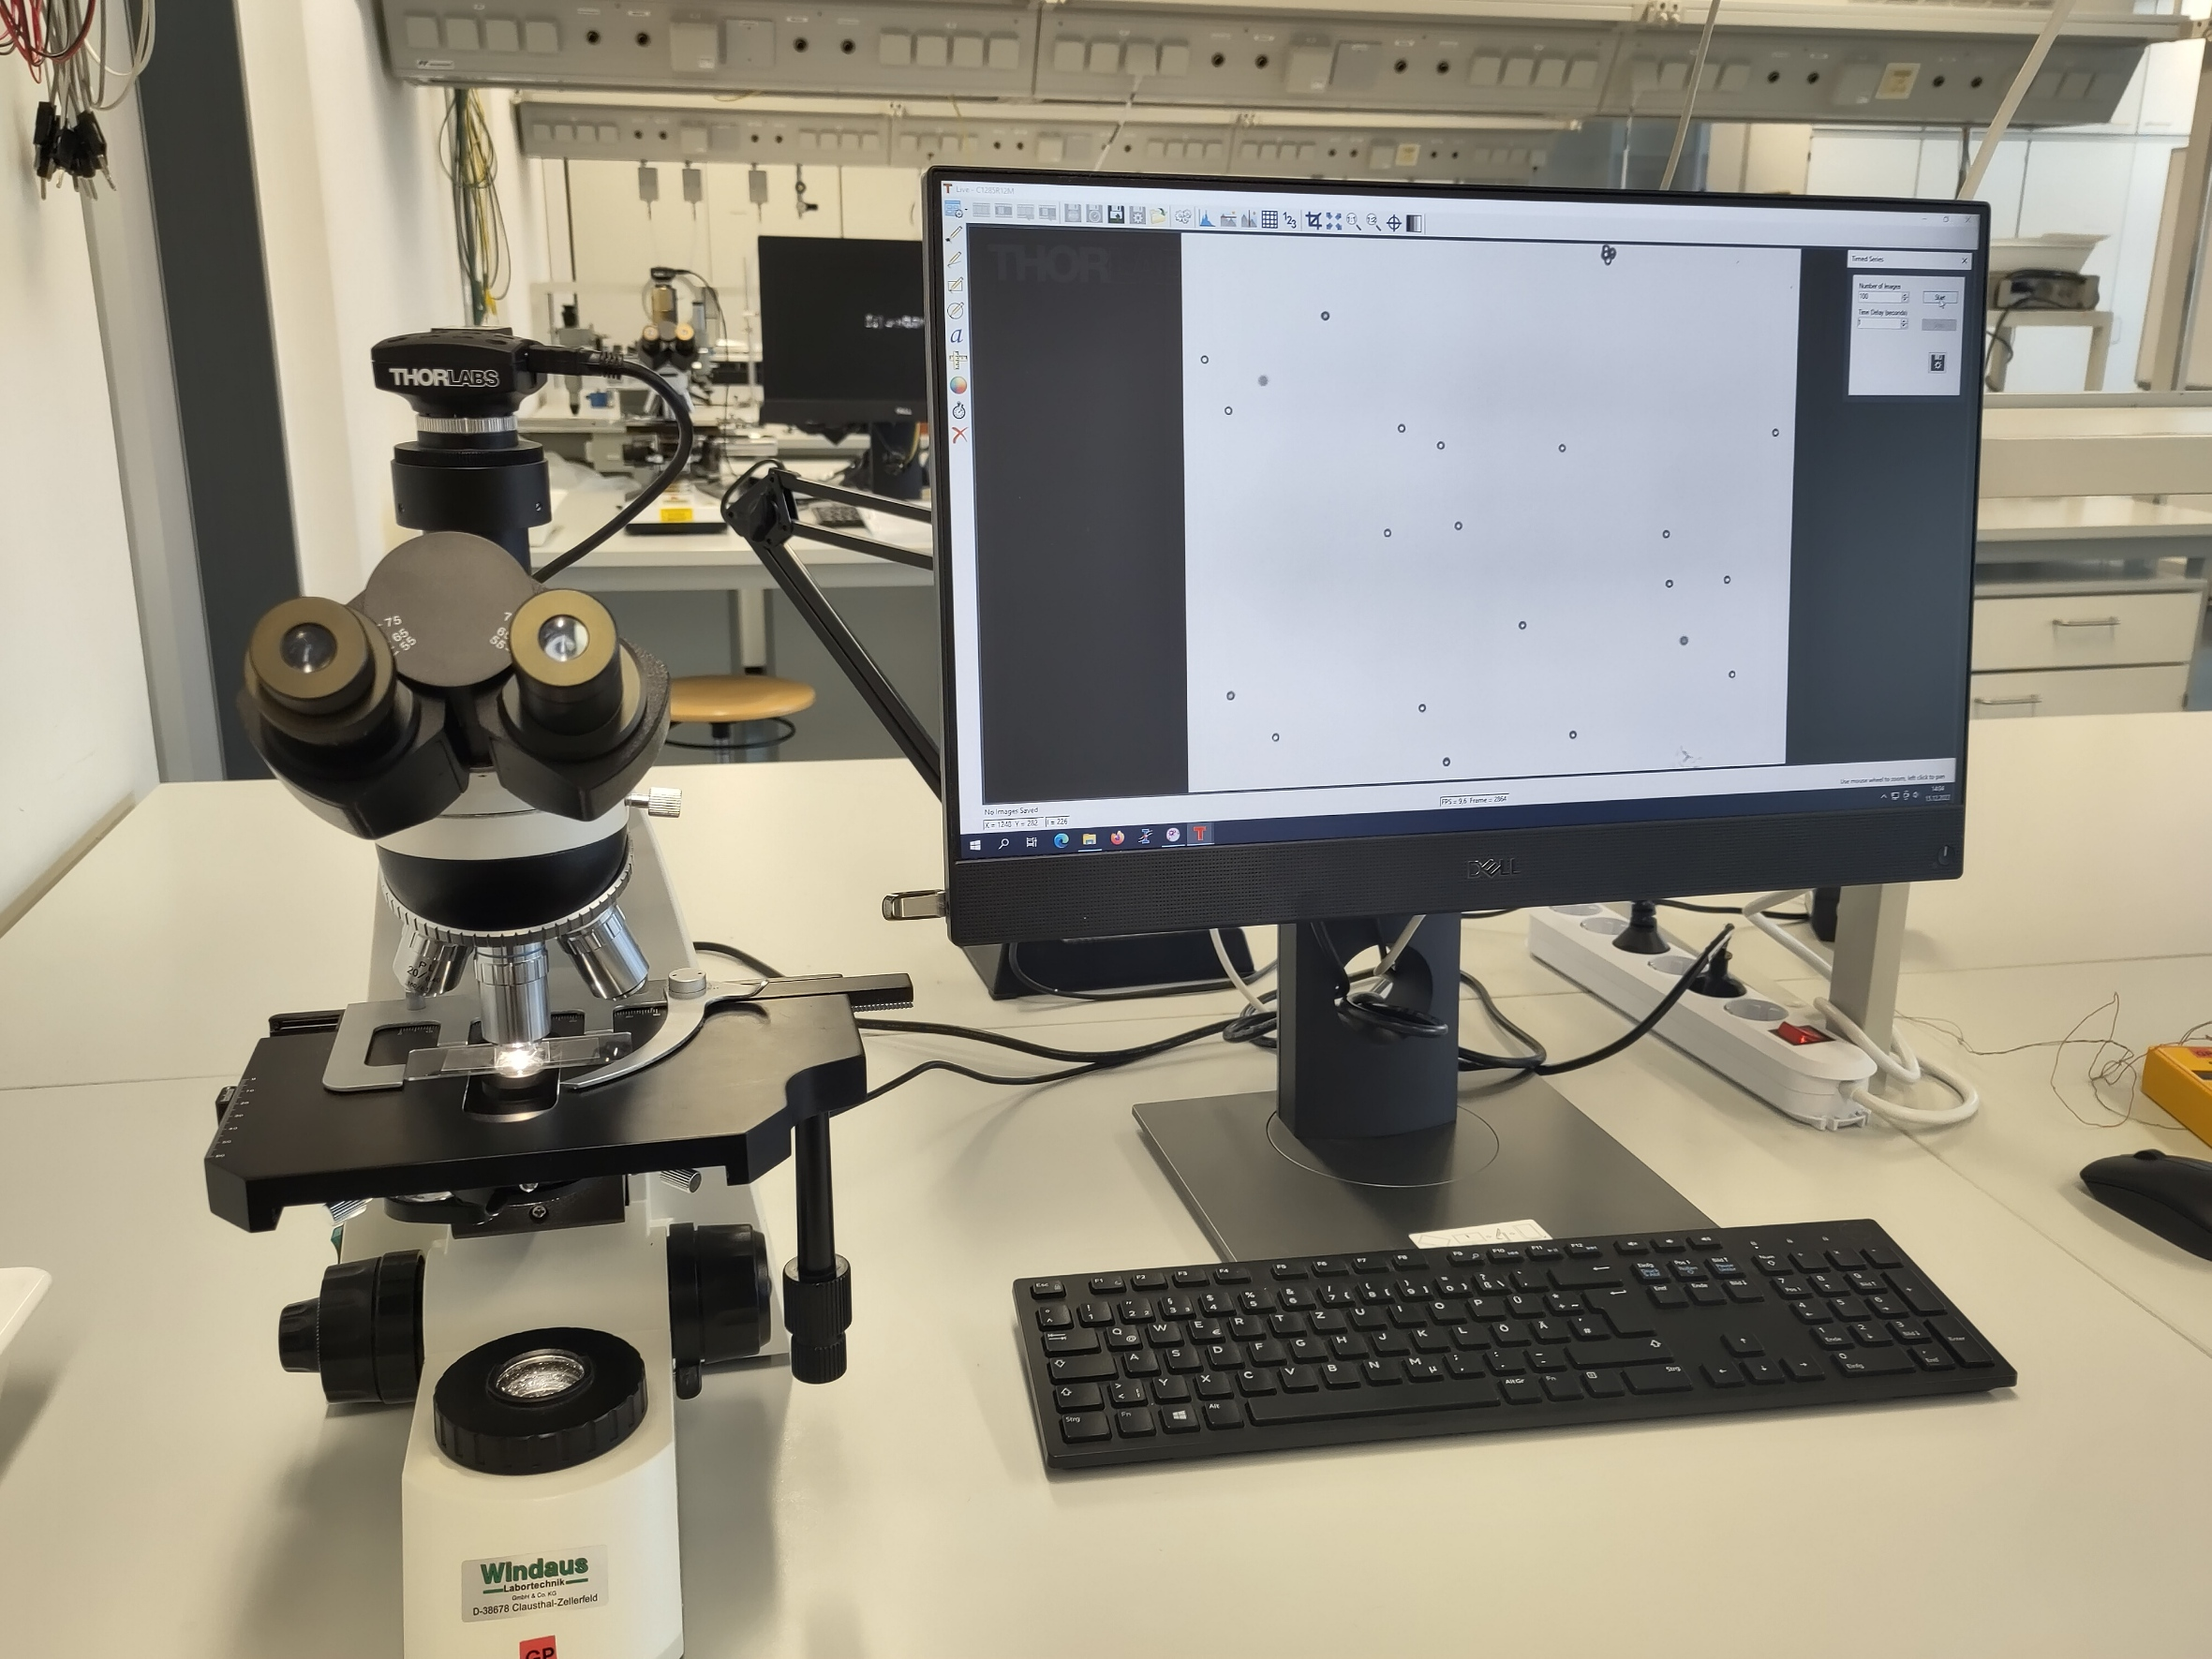
\includegraphics{"Bilder/Versuchsaufbau.png"}
\caption{Versuchsaufbau}
\end{figure}

Zu Beginn des eigentlichen Versuches wird die Raumtemperatur gemessen.

Im Messzylinder werden 100ml und 70 ml Wasser abgemessen und
anschließend in das Kaloriemeter gefüllt. In diesem Zustand wird dessen
Masse gemessen. Der Deckel des Kaloriemeters mit Heizspirale,
Thermometer und Rührstab wird geschlossen. Die Heizspirale wird über
Bananenstecker mit dem AC Netzgerät verbunden. Ein Amperemeter wird in
Reihe und ein Voltmeter parallel geschaltet.

Am Netzgerät wird eine mittlere Leistung eingestellt (50\%) und über den
Zeitraum von sieben Minuten eine Temperatur-Zeit Messreihe aufgenommen.
Während dieser Zeit wird zudem immer wieder die Spannung und die
Stromstärke kontrolliert, die das Kaloriemeter durchfließt
beziehungsweise die an der Heizspirale anliegt.

\hypertarget{fehlerbetrachtung}{%
\subsection{Fehlerbetrachtung}\label{fehlerbetrachtung}}

\hypertarget{beobachtungen}{%
\subsection{Beobachtungen}\label{beobachtungen}}

Die Erhitzung im Kaloriemeter zeigt folgenden Temperaturverlauf:

\begin{Shaded}
\begin{Highlighting}[]
\CommentTok{\# Einlesen der csv{-}Datei}
\NormalTok{zeitreiheErhitzung }\OtherTok{\textless{}{-}} \FunctionTok{read.csv}\NormalTok{(}\StringTok{"Daten/Messreihe.csv"}\NormalTok{, }\AttributeTok{sep =} \StringTok{";"}\NormalTok{, }\AttributeTok{dec=}\StringTok{","}\NormalTok{)}
\CommentTok{\# Tidy{-}up}
\NormalTok{zeitreiheErhitzung }\OtherTok{\textless{}{-}}\NormalTok{ zeitreiheErhitzung[}\DecValTok{2}\SpecialCharTok{:}\FunctionTok{nrow}\NormalTok{(zeitreiheErhitzung), }\DecValTok{10}\SpecialCharTok{:}\DecValTok{11}\NormalTok{]}
\FunctionTok{colnames}\NormalTok{(zeitreiheErhitzung) }\OtherTok{\textless{}{-}} \FunctionTok{c}\NormalTok{(}\StringTok{"Zeit\_s"}\NormalTok{, }\StringTok{"Temperatur"}\NormalTok{)}

\CommentTok{\# Lineare Regression}
\NormalTok{lm }\OtherTok{\textless{}{-}} \FunctionTok{lm}\NormalTok{(zeitreiheErhitzung}\SpecialCharTok{$}\NormalTok{Temperatur}\SpecialCharTok{\textasciitilde{}}\NormalTok{zeitreiheErhitzung}\SpecialCharTok{$}\NormalTok{Zeit\_s)}
\CommentTok{\# Steigung a extrahieren}
\NormalTok{a }\OtherTok{\textless{}{-}}\NormalTok{ lm}\SpecialCharTok{$}\NormalTok{coefficient[}\DecValTok{2}\NormalTok{]}
\CommentTok{\# Y{-}Achsenabschnitt b extrahieren}
\NormalTok{b }\OtherTok{\textless{}{-}}\NormalTok{ lm}\SpecialCharTok{$}\NormalTok{coefficient[}\DecValTok{1}\NormalTok{]}
\CommentTok{\# Standardfehler R\^{}2 extrahieren}
\NormalTok{lmsummary }\OtherTok{\textless{}{-}} \FunctionTok{summary}\NormalTok{(lm)}
\NormalTok{R }\OtherTok{\textless{}{-}}\NormalTok{ lmsummary}\SpecialCharTok{$}\NormalTok{coefficients[}\DecValTok{2}\NormalTok{,}\DecValTok{2}\NormalTok{]}

\CommentTok{\# Ausgabe als Plot}
\NormalTok{\{}\FunctionTok{plot}\NormalTok{(}\AttributeTok{x=}\NormalTok{zeitreiheErhitzung}\SpecialCharTok{$}\NormalTok{Zeit\_s, }\AttributeTok{y=}\NormalTok{zeitreiheErhitzung}\SpecialCharTok{$}\NormalTok{Temperatur,}
      \CommentTok{\# Aesthetics}
      \AttributeTok{ylab =} \StringTok{"Temperatur T in °C"}\NormalTok{,}
      \AttributeTok{xlab =} \StringTok{"Zeit t in s"}\NormalTok{,}
      \AttributeTok{main=} \StringTok{"Temperaturverlauf im Kaloriemeter"}\NormalTok{,}
      \AttributeTok{pch=}\DecValTok{20}\NormalTok{, }\AttributeTok{las=}\DecValTok{1}\NormalTok{)}
  \CommentTok{\# Einzeichnen der Regressionsgeraden}
  \FunctionTok{abline}\NormalTok{(}\AttributeTok{coef=}\FunctionTok{c}\NormalTok{(b, a))}
  \CommentTok{\# Einzeichen der Regressiosgeraden ab{-}/zuzüglich des Fehlers}
  \FunctionTok{abline}\NormalTok{(}\AttributeTok{coef=}\FunctionTok{c}\NormalTok{(b, a}\SpecialCharTok{{-}}\NormalTok{R))}
  \FunctionTok{abline}\NormalTok{(}\AttributeTok{coef=}\FunctionTok{c}\NormalTok{(b, a}\SpecialCharTok{+}\NormalTok{R))}
  \CommentTok{\# Legendenerzeugung}
  \FunctionTok{legend}\NormalTok{(}\AttributeTok{x=}\DecValTok{270}\NormalTok{, }\AttributeTok{y=}\NormalTok{(}\FloatTok{0.98}\SpecialCharTok{*}\FunctionTok{max}\NormalTok{(zeitreiheErhitzung}\SpecialCharTok{$}\NormalTok{Temperatur)), }
         \AttributeTok{legend=}\FunctionTok{c}\NormalTok{(}\StringTok{"Messwerte"}\NormalTok{, }\FunctionTok{paste}\NormalTok{(}\StringTok{"Lineare Regression:"}\NormalTok{,}
                                     \StringTok{"}\SpecialCharTok{\textbackslash{}n}\StringTok{y=ax+b"}\NormalTok{,}
                                     \StringTok{"}\SpecialCharTok{\textbackslash{}n}\StringTok{a = "}\NormalTok{, }\FunctionTok{round}\NormalTok{(a,}\DecValTok{5}\NormalTok{), }
                                     \StringTok{"}\SpecialCharTok{\textbackslash{}n}\StringTok{b = "}\NormalTok{, }\FunctionTok{round}\NormalTok{(b,}\DecValTok{3}\NormalTok{),}
                                     \StringTok{"}\SpecialCharTok{\textbackslash{}n}\StringTok{R\^{}2 = "}\NormalTok{, }\FunctionTok{round}\NormalTok{(R, }\DecValTok{5}\NormalTok{))),}
         \AttributeTok{col=}\StringTok{"black"}\NormalTok{, }\AttributeTok{pch =} \FunctionTok{c}\NormalTok{(}\DecValTok{20}\NormalTok{, }\DecValTok{26}\NormalTok{), }\AttributeTok{lty=}\FunctionTok{c}\NormalTok{(}\DecValTok{0}\NormalTok{,}\DecValTok{1}\NormalTok{),}
         \AttributeTok{bty =} \StringTok{"n"}\NormalTok{)}
\NormalTok{\}}
\end{Highlighting}
\end{Shaded}

\begin{verbatim}
## Warning in plot.xy(xy.coords(x, y), type = type, ...): nicht implementierter
## Wert '26' für pch
\end{verbatim}

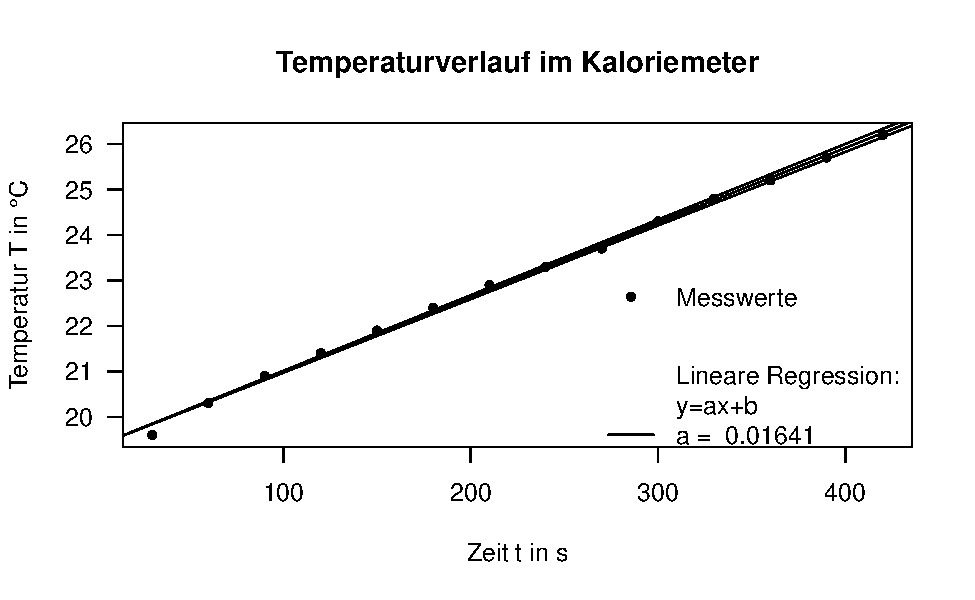
\includegraphics{Kaloriemeter_files/figure-latex/unnamed-chunk-1-1.pdf}
\emph{Abb. 1: Für sieben Minuten wurde der Temperaturverlauf der
Erhitzung des Wassers im Kaloriemeter gemessen}

Der Temperaturverlauf macht im betrachteten Zeitraum einen linearen
Eindruck. Eine Regressionsgerade hat die Steigung
\(a=(1641\pm 22)\cdot 10^{-5}\ ^{\circ} C\ s^{-1}\)

\hypertarget{auswertung}{%
\subsection{Auswertung}\label{auswertung}}

\hypertarget{interpretation}{%
\subsection{Interpretation}\label{interpretation}}

\hypertarget{versuch-2}{%
\section{Versuch 2}\label{versuch-2}}

\hypertarget{thema-1}{%
\subsection{Thema}\label{thema-1}}

\hypertarget{versuchsaufbau}{%
\subsection{Versuchsaufbau}\label{versuchsaufbau}}

``\,''

\hypertarget{durchfuxfchrung}{%
\subsection{Durchführung}\label{durchfuxfchrung}}

\hypertarget{fehlerbetrachtung-1}{%
\subsection{Fehlerbetrachtung}\label{fehlerbetrachtung-1}}

\hypertarget{beobachtungen-1}{%
\subsection{Beobachtungen}\label{beobachtungen-1}}

Oranges Metall: Durchmesser\_Groß: 2,49cm Durchmesser\_klein: 0,58cm
Höhe\_groß: 4,52mm Höhe\_klein: 0,815mm Masse: 198,0g

Graues Metall: Durchmesser\_Groß: 2,50cm Durchmesser\_klein:0,635
Höhe\_groß:4,515cm Höhe\_klein:0,85mm Masse: 176,12

\hypertarget{wasserverdruxe4ngung}{%
\section{Wasserverdrängung}\label{wasserverdruxe4ngung}}

Orangenes Metall:

\begin{Shaded}
\begin{Highlighting}[]
\DecValTok{58{-}35}
\end{Highlighting}
\end{Shaded}

\begin{verbatim}
## [1] 23
\end{verbatim}

Graues Metall:

\begin{Shaded}
\begin{Highlighting}[]
\DecValTok{57{-}35}
\end{Highlighting}
\end{Shaded}

\begin{verbatim}
## [1] 22
\end{verbatim}

\hypertarget{oranges-metall}{%
\section{Oranges Metall}\label{oranges-metall}}

\hypertarget{wassermasse}{%
\section{Wassermasse}\label{wassermasse}}

Wassermasse mit Becherglas:235,5g Becherglas leer: 97,4g Wassermasse
ohne Becherglas: T\_A (Warmes Wasser): 50,0°C T\_B (Mischtemp):
(vorläufig 46,1°C) (dann 44,9) (eigeloggt: 44,2g)

\hypertarget{graues-metall}{%
\section{Graues Metall}\label{graues-metall}}

Wassermasse mit Becherglas:241,3g Wassermasse ohne Becherglas: T\_A
(Warmes Wasser): 49,1°C T\_B (Mischtemp): (vorläufig 44,1°C) (dann 43,4)
(eigeloggt 42,8)

\hypertarget{auswertung-1}{%
\subsection{Auswertung}\label{auswertung-1}}

\hypertarget{interpretation-1}{%
\subsection{Interpretation}\label{interpretation-1}}

\end{document}
